\PassOptionsToPackage{unicode=true}{hyperref} % options for packages loaded elsewhere
\PassOptionsToPackage{hyphens}{url}
%
\documentclass[lettepaper,]{article}
\usepackage{lmodern}
\usepackage{amssymb,amsmath}
\usepackage{ifxetex,ifluatex}
\usepackage{fixltx2e} % provides \textsubscript
\ifnum 0\ifxetex 1\fi\ifluatex 1\fi=0 % if pdftex
  \usepackage[T1]{fontenc}
  \usepackage[utf8]{inputenc}
  \usepackage{textcomp} % provides euro and other symbols
\else % if luatex or xelatex
  \usepackage{unicode-math}
  \defaultfontfeatures{Ligatures=TeX,Scale=MatchLowercase}
\fi
% use upquote if available, for straight quotes in verbatim environments
\IfFileExists{upquote.sty}{\usepackage{upquote}}{}
% use microtype if available
\IfFileExists{microtype.sty}{%
\usepackage[]{microtype}
\UseMicrotypeSet[protrusion]{basicmath} % disable protrusion for tt fonts
}{}
\IfFileExists{parskip.sty}{%
\usepackage{parskip}
}{% else
\setlength{\parindent}{0pt}
\setlength{\parskip}{6pt plus 2pt minus 1pt}
}
\usepackage{hyperref}
\hypersetup{
            pdftitle={Finding Foundations},
            pdfauthor={Jack Beasley, jbeasley@stanford.edu; Kristine Guo, kguo98@stanford.edu},
            pdfborder={0 0 0},
            breaklinks=true}
\urlstyle{same}  % don't use monospace font for urls
\usepackage[margin=1in]{geometry}
\usepackage{color}
\usepackage{fancyvrb}
\newcommand{\VerbBar}{|}
\newcommand{\VERB}{\Verb[commandchars=\\\{\}]}
\DefineVerbatimEnvironment{Highlighting}{Verbatim}{commandchars=\\\{\}}
% Add ',fontsize=\small' for more characters per line
\newenvironment{Shaded}{}{}
\newcommand{\AlertTok}[1]{\textcolor[rgb]{1.00,0.00,0.00}{\textbf{#1}}}
\newcommand{\AnnotationTok}[1]{\textcolor[rgb]{0.38,0.63,0.69}{\textbf{\textit{#1}}}}
\newcommand{\AttributeTok}[1]{\textcolor[rgb]{0.49,0.56,0.16}{#1}}
\newcommand{\BaseNTok}[1]{\textcolor[rgb]{0.25,0.63,0.44}{#1}}
\newcommand{\BuiltInTok}[1]{#1}
\newcommand{\CharTok}[1]{\textcolor[rgb]{0.25,0.44,0.63}{#1}}
\newcommand{\CommentTok}[1]{\textcolor[rgb]{0.38,0.63,0.69}{\textit{#1}}}
\newcommand{\CommentVarTok}[1]{\textcolor[rgb]{0.38,0.63,0.69}{\textbf{\textit{#1}}}}
\newcommand{\ConstantTok}[1]{\textcolor[rgb]{0.53,0.00,0.00}{#1}}
\newcommand{\ControlFlowTok}[1]{\textcolor[rgb]{0.00,0.44,0.13}{\textbf{#1}}}
\newcommand{\DataTypeTok}[1]{\textcolor[rgb]{0.56,0.13,0.00}{#1}}
\newcommand{\DecValTok}[1]{\textcolor[rgb]{0.25,0.63,0.44}{#1}}
\newcommand{\DocumentationTok}[1]{\textcolor[rgb]{0.73,0.13,0.13}{\textit{#1}}}
\newcommand{\ErrorTok}[1]{\textcolor[rgb]{1.00,0.00,0.00}{\textbf{#1}}}
\newcommand{\ExtensionTok}[1]{#1}
\newcommand{\FloatTok}[1]{\textcolor[rgb]{0.25,0.63,0.44}{#1}}
\newcommand{\FunctionTok}[1]{\textcolor[rgb]{0.02,0.16,0.49}{#1}}
\newcommand{\ImportTok}[1]{#1}
\newcommand{\InformationTok}[1]{\textcolor[rgb]{0.38,0.63,0.69}{\textbf{\textit{#1}}}}
\newcommand{\KeywordTok}[1]{\textcolor[rgb]{0.00,0.44,0.13}{\textbf{#1}}}
\newcommand{\NormalTok}[1]{#1}
\newcommand{\OperatorTok}[1]{\textcolor[rgb]{0.40,0.40,0.40}{#1}}
\newcommand{\OtherTok}[1]{\textcolor[rgb]{0.00,0.44,0.13}{#1}}
\newcommand{\PreprocessorTok}[1]{\textcolor[rgb]{0.74,0.48,0.00}{#1}}
\newcommand{\RegionMarkerTok}[1]{#1}
\newcommand{\SpecialCharTok}[1]{\textcolor[rgb]{0.25,0.44,0.63}{#1}}
\newcommand{\SpecialStringTok}[1]{\textcolor[rgb]{0.73,0.40,0.53}{#1}}
\newcommand{\StringTok}[1]{\textcolor[rgb]{0.25,0.44,0.63}{#1}}
\newcommand{\VariableTok}[1]{\textcolor[rgb]{0.10,0.09,0.49}{#1}}
\newcommand{\VerbatimStringTok}[1]{\textcolor[rgb]{0.25,0.44,0.63}{#1}}
\newcommand{\WarningTok}[1]{\textcolor[rgb]{0.38,0.63,0.69}{\textbf{\textit{#1}}}}
\usepackage{longtable,booktabs}
% Fix footnotes in tables (requires footnote package)
\IfFileExists{footnote.sty}{\usepackage{footnote}\makesavenoteenv{longtable}}{}
\usepackage{graphicx,grffile}
\makeatletter
\def\maxwidth{\ifdim\Gin@nat@width>\linewidth\linewidth\else\Gin@nat@width\fi}
\def\maxheight{\ifdim\Gin@nat@height>\textheight\textheight\else\Gin@nat@height\fi}
\makeatother
% Scale images if necessary, so that they will not overflow the page
% margins by default, and it is still possible to overwrite the defaults
% using explicit options in \includegraphics[width, height, ...]{}
\setkeys{Gin}{width=\maxwidth,height=\maxheight,keepaspectratio}
\setlength{\emergencystretch}{3em}  % prevent overfull lines
\providecommand{\tightlist}{%
  \setlength{\itemsep}{0pt}\setlength{\parskip}{0pt}}
\setcounter{secnumdepth}{0}
% Redefines (sub)paragraphs to behave more like sections
\ifx\paragraph\undefined\else
\let\oldparagraph\paragraph
\renewcommand{\paragraph}[1]{\oldparagraph{#1}\mbox{}}
\fi
\ifx\subparagraph\undefined\else
\let\oldsubparagraph\subparagraph
\renewcommand{\subparagraph}[1]{\oldsubparagraph{#1}\mbox{}}
\fi

% set default figure placement to htbp
\makeatletter
\def\fps@figure{htbp}
\makeatother

\usepackage{booktabs}

\title{Finding Foundations}
\author{Jack Beasley, \texttt{jbeasley@stanford.edu} \and Kristine Guo, \texttt{kguo98@stanford.edu}}
\date{October 18th, 2018}

\begin{document}
\maketitle
\begin{abstract}
An important task in the domain of citation network analysis concerns
discovering and understanding the development of academic knowledge
throughout time. Previous research has made great strides in
understanding the structures of academia, but the results are limited to
narrowly-defined concepts and rely on domain-specific datasets.

In this paper, we aim to discover trends and structures of research
development in academia for a broad range of domains. To do so, we use a
very large general citation network, the Microsoft Academic Graph (MAG),
instead of relying on a domain-specific dataset. Using this network, we
aim to identify the lineage of papers that have laid the foundations for
the development of any given paper in the MAG.

The proposed system has two distinct parts. First, we utilize
breadth-first search from the paper in question to create a domain
specific dataset in real-time. Notably, this algorithm works around the
limitation that the MAG is larger than the researchers' available system
memory, effectively allowing users to partition a large graph on a
laptop or inexpensive server without a lot of memory. Secondly, we use
citation network analysis techniques to identify the ``lineage'' of a
work, which we take to be series of works that capture the given paper's
path of academic development and foundations. In particular, we evaluate
the performance and distinctive characteristics of several algorithms,
including main path analysis, betweenness centrality, and PageRank.

Through our findings, we demonstrate a potential method for tracing the
academic lineage of arbitrary works on large citation networks using
inexpensive hardware.
\end{abstract}

\hypertarget{introduction}{%
\section{Introduction}\label{introduction}}

Citation network analysis offers a wealth of information about
professional communities and the development of academic research. One
common application of this information is to create recommendation
systems that can refer readers to other relevant sources. To do so,
extensive research has been conducted to craft robust methods that
attempt to determine which papers are most important and impactful
within a given field.

However, rather than identify papers that are generally popular in a
field, in this paper we are concerned with finding papers that are
foundational specifically to the development of a single paper at hand.
Thus, we aim to build a recommendation system that can discover the
papers that have most directly contributed to the knowledge any given
paper builds on.

To accomplish this task, recent research has employed methods of
citation network analysis in order to examine the evolutionary structure
of academic knowledge throughout time. However, such findings are often
limited to narrowly-defined scientific concepts and fields,\footnote{Calero-Medina
  and Noyons, ``Combining Mapping and Citation Network Analysis for a
  Better Understanding of the Scientific Development,''
  @liuIntegratedApproachMain2012, @xiaoKnowledgeDiffusionPath2014.}
require manual curation of domain-specific citation datasets, and fail
to apply to the broader day-to-day inquiries a researcher may have.

Thus, the key contribution of our work is applying methods of network
analysis to a large, comprehensive citation dataset, allowing
exploration of almost every domain of academia. In order to handle a
citation network of this magnitude, we craft algorithms for extracting
any paper's local neighborhood in the citation network in an efficient
manner such that recommendations can feasibly be returned to a user
interactively. Finally, we apply variations of main path analysis in
order to trace the academic lineage for the given paper based on its
local neighborhood of citations and references.

Thus, the contributions of our paper extend previous work by abstracting
their methods and results to operate on papers from any field, not
simply a small subfield, while also removing the need for manual
construction of domain-specific datasets. By doing so, we hope to make
the evolutionary structure of academic research more accessible for
anyone attempting to gain a broad understanding of the development of
academic literature.

\hypertarget{related-work}{%
\section{Related Work}\label{related-work}}

\hypertarget{single-score-methods}{%
\subsection{Single-Score Methods}\label{single-score-methods}}

There exist many different methods to determine node importance in a
graph. For paper and journal importance applications, Clarivate
Analytics has published journal importance statistics based on two
distinct measures: the Journal Impact Factor, which is mostly based on
citation counts\footnote{``Impact Factor - Clarivate.''} and the
Eigenfactor score,\footnote{Bergstrom, West, and Wiseman, ``The
  Eigenfactor™ Metrics.''} which is essentially a modified PageRank
algorithm for citation networks rather than web networks.

While these methods provide effective rankings given the properties they
attempt to rank by, they provide nothing but a single score number that
can be hard to interpret. Because these scores distill complex graph
phenomena into a single number, they offer little help in determining
the actual relationships between articles and understanding the larger
development of science. Thus, single-score methods do not effectively
help researchers with the problem of determining what the foundations of
a paper are.

Because of this lack of information from single-score methods, we seek
algorithms that preserve the citation network graph structure. Thus, our
research pointed us towards the usage of main path analysis, which we
will explore more in the next three papers.

\hypertarget{combining-mapping-and-citation-network-analysis-for-a-better-understanding-of-the-scientific-development-calero-medinacombiningmappingcitation2008}{%
\subsection[Combining mapping and citation network analysis for a better
understanding of the scientific development]{\texorpdfstring{Combining
mapping and citation network analysis for a better understanding of the
scientific development\footnote{Calero-Medina and Noyons, ``Combining
  Mapping and Citation Network Analysis for a Better Understanding of
  the Scientific Development.''}}{Combining mapping and citation network analysis for a better understanding of the scientific development}}\label{combining-mapping-and-citation-network-analysis-for-a-better-understanding-of-the-scientific-development-calero-medinacombiningmappingcitation2008}}

Calero-Medina and Noyons combine bibliometric mapping and citation
network analysis in order to investigate the development of scientific
knowledge about Absorptive Capacity, a term coined in 1988 that has had
widespread influence on the field of Organization.

For citation network analysis in particular, they utilize two different
methods: 1) main path analysis, and 2) hubs and authorities analysis.
Main path analysis identifies the nodes that are most frequently used in
``walks'' from the most recent citations to the oldest. By computing all
such possible paths, we can discover the papers that are more frequently
encountered throughout time, pointing towards their centrality in the
development of an academic specialization. This technique is combined
with information gained from using hubs and authorities analysis, which
identifies papers that are both cited by other prominent papers as well
as cite important papers themselves.

By combining these different perspectives, Calero-Medina and Noyons
successfully identify 15 papers that comprise the main path component of
the Absorptive Capacity field. Thus, this paper provides inspiration for
using main path analysis to identify foundational papers in combination
with hubs and authorities which actually ranks and scores the papers.

\hypertarget{an-integrated-approach-for-main-path-analysis-development-of-the-hirsch-index-as-an-example-liuintegratedapproachmain2012}{%
\subsection[An integrated approach for main path analysis: Development
of the Hirsch index as an example]{\texorpdfstring{An integrated
approach for main path analysis: Development of the Hirsch index as an
example\footnote{Liu and Lu, ``An Integrated Approach for Main Path
  Analysis.''}}{An integrated approach for main path analysis: Development of the Hirsch index as an example}}\label{an-integrated-approach-for-main-path-analysis-development-of-the-hirsch-index-as-an-example-liuintegratedapproachmain2012}}

Liu and Lu begin by critiquing the technique of main path analysis. The
original main path analysis only identifies a single main path, which is
not representative of larger scientific networks that often have
multiple main paths. Furthermore, the original algorithm greedily
constructs the main path by repeatedly selecting the link with the
highest search path count (SPC). However, as with many greedy
algorithms, this algorithm is not guaranteed to produce the path with
the largest cumulative SPC or contain the link with the largest SPC.

Therefore, Liu and Lu propose new variations on main path analysis. For
example, global main path analysis aims to find the path with the true
overall largest SPC. Another is multiple main path analysis, which
identifies multiple local main paths by relaxing the search constraints
to reveal more detailed information. Finally, key-route main path
analysis guarantees that the link with the highest SPC is included by
beginning the search from both ends of the link instead of the source
nodes. Importantly, all of these methods can be combined as well.

Thus, the authors next apply an integrated approach that utilizes a
combination of main path analysis methods in order to examine the
development of the Hirsch index. Ultimately, their results prove that
the main path analyses developed by Liu and Lu enhance our capability to
capture different types of information about the relationships between
scientific articles.

\hypertarget{knowledge-diffusion-path-analysis-of-data-quality-literature-a-main-path-analysis-xiaoknowledgediffusionpath2014}{%
\subsection[Knowledge diffusion path analysis of data quality
literature: A main path analysis]{\texorpdfstring{Knowledge diffusion
path analysis of data quality literature: A main path analysis\footnote{Xiao
  et al., ``Knowledge Diffusion Path Analysis of Data Quality
  Literature.''}}{Knowledge diffusion path analysis of data quality literature: A main path analysis}}\label{knowledge-diffusion-path-analysis-of-data-quality-literature-a-main-path-analysis-xiaoknowledgediffusionpath2014}}

In this article, Xiao et al.~integrate local, global, multiple-global,
and key-route main path analyses to uncover knowledge diffusion paths of
data quality literature. In particular, they demonstrate that each type
of main path analysis reveals different yet complementary information
about development trends.

For example, local and global main path analysis highlight the papers
that have provided major contributions to the field. On the other hand,
multiple global and the key-route main path analyses provide more
complete pictures of development trends by identifying multiple paths,
revealing the divergence-convergence of the citation network as it
evolves throughout time.

Finally, and perhaps most importantly, Xiao et al.~also provide
intuitive graphical representations of main path analyses in order to
both convey their nuances and allow the reader to view the
interrelationships between papers. This method of presenting results in
particular serves as an inspiration for our project.

\hypertarget{motivation-for-improvement}{%
\subsection{Motivation for
Improvement}\label{motivation-for-improvement}}

As seen from the literature review above, citation network and main path
analysis are often limited to characterizing the development structures
of specific concepts and subfields such as Absorptive Capacity, the
Hirsch Index, and data quality literature.

This reality proves less than ideal for researchers and academics, who
are told to ``stand on the shoulders of giants'' but are not given any
tools that they can use to efficiently peruse and explore the
development of their field. For example, conducting a literature review
requires the ability to determine what works constitute essential
background reading for a given paper, as well as assessing works with
large impact when attempting to create new innovational methods.

However, this is not an easy process, as making literature reviews is a
time-consuming manual problem that consists of recursively searching
through papers' citations to try to understand what actual authorities
and ground truths underlie a research problem. Beyond even just
academics, people with casual interest in a field should also be able to
have easy access to a field's literature without having to manually
search for its most foundational papers. Such tasks would benefit from
comprehensive knowledge of the development of the techniques and
concepts under question.

\hypertarget{dataset}{%
\section{Dataset}\label{dataset}}

While there are many options for citation networks, for this project we
selected the Microsoft Academic Graph (MAG)\footnote{Sinha et al., ``An
  Overview of Microsoft Academic Service (MAS) and Applications.''}. We
chose this dataset because it is
\href{https://docs.microsoft.com/en-us/academic-services/graph/get-started-setup-provisioning\#open-data-license-odc-by}{freely
available under an open license}, and it has also been described as
``the most comprehensive publicly available dataset of its kind'' in a
review article.\footnote{Herrmannova and Knoth, ``An Analysis of the
  Microsoft Academic Graph.''}

We initially chose the 2017 snapshot of the MAG
\href{https://www.openacademic.ai/oag/}{made available by the Open
Academic Society}, however, the IDs assigned to papers in that dataset
do not match those used by the
\href{https://labs.cognitive.microsoft.com/en-us/project-academic-knowledge}{Microsoft
Academic API}, meaning that looking up paper titles from IDs required a
local copy of the entire uncompressed dataset which totalled 300GB.

Thus, we instead contacted Microsoft and got access to a recent snapshot
(accurate as of 2018-10-12) of the current MAG. We then downloaded only
the
\href{https://docs.microsoft.com/en-us/academic-services/graph/reference-data-schema\#paperreferencestxt}{PaperReferences}
file, which is a 31.3 GB edge list, where paper IDs are 64-bit integers.

\hypertarget{inexpensively-constructing-local-neighborhoods}{%
\section{Inexpensively Constructing Local
Neighborhoods}\label{inexpensively-constructing-local-neighborhoods}}

\hypertarget{motivation}{%
\subsection{Motivation}\label{motivation}}

As explained above, due to its large, comprehensive dataset of
citations, we utilize the Microsoft Academic Graph (MAG) as our
principal citation network in order to be able to apply our methods to
any paper within the MAG. However, using the MAG poses a challenge due
principally to the large size of the dataset.

The MAG contains an edge list of 1,269,744,602 edges, each consisting of
two 64-bit integer ids. Consequently, fitting the whole edgelist in
memory would require a machine with at least 22 GB of RAM, plus more RAM
for auxiliary data structures. Given the limited nature of the computing
hardware available (laptops with 8GB of RAM and compute credits for
cloud instances with 4GB of RAM), we could not simply load the dataset
into memory and perform a typical breadth-first search.

Thus, we devised a system to quickly run breadth-first search such that
we minimize lookups to the edge list on the HDD or SSD while minimizing
memory usage. This work follows a similar vein as GraphChi\footnote{Kyrola,
  Blelloch, and Guestrin, ``GraphChi.''} or X-Stream,\footnote{Roy,
  Mihailovic, and Zwaenepoel, ``X-Stream.''} but specifically designed
for the specific task of subgraph partitioning rather than more general
graph computation frameworks. Notably, this algorithm still makes the
assumption that while the whole graph cannot fit in RAM, a given paper's
subgraph can.

\hypertarget{method}{%
\subsection{Method}\label{method}}

Our method has two distinct phases: hashing and traversal. In the
hashing step, we create two indexes by hashing edges to files based on
the source node id for the first and the destination node id for the
second. This method is similar to the ``shard'' method employed by
GraphChi as each shard contains a number of edges that can can be fully
loaded into memory. However, to simplify implementation, we hashed to
separate files, rather than sorting the list into shards.

\begin{Shaded}
\begin{Highlighting}[]
\KeywordTok{func}\NormalTok{ hashEdgeList(source, srcHashFolder, dstHashFolder, numberHashFiles)\{}
    \KeywordTok{for}\NormalTok{ line := }\KeywordTok{range}\NormalTok{ source \{}
\NormalTok{        sourceID, destinationID <- line}
\NormalTok{        srcHashFolder$\{sourceID % numberHashFiles\} <- line}
\NormalTok{        dstHashFolder$\{destinationID % numberHashFiles\} <- line}
\NormalTok{    \}}
\NormalTok{\}}
\end{Highlighting}
\end{Shaded}

Once we have pre-processed and hashed the data, we can use that data
structure to traverse the graph in pieces.

\begin{Shaded}
\begin{Highlighting}[]
\KeywordTok{func}\NormalTok{ BFSOutLinks(initialPaperID, levels, output)\{}
\NormalTok{    seenPapers := Set()}
\NormalTok{    seenPapers.Add(initialPaperID)}
\NormalTok{    currentPapers := Set()}
\NormalTok{    currentPapers.Add(initialPaperID)}

    \KeywordTok{for}\NormalTok{ i <- \{}\DecValTok{0}\NormalTok{, …, levels\} \{}
\NormalTok{        nextPapers := Set()}
        \KeywordTok{for}\NormalTok{ id <- currentPapers \{}
            \KeywordTok{for}\NormalTok{ line <- srcHashFolder$\{id % numberHashFiles\} \{}
\NormalTok{                sourceID, destinationID <- line}
                \KeywordTok{if}\NormalTok{ currentPapers.Contains(sourceID) && !seenPapers.Contains(destinationID) \{}
\NormalTok{                    seenPapers.Add(destinationID)}
\NormalTok{                    nextPapers.Add(destinationID)}
\NormalTok{                    output <- line}
\NormalTok{                \}}
\NormalTok{            \}}
\NormalTok{        \}}
\NormalTok{        currentPapers = nextPapers}
\NormalTok{    \}}
\NormalTok{\}}
\end{Highlighting}
\end{Shaded}

The BFS maintains a set of currentPapers and of seenPapers. The
currentPapers set keeps track of all the starting points for the next
level of BFS and is cleared at the end of each level. The seenNodes set
contains all nodes previously seen by the BFS. Thus, this set results on
the majority of memory use for the algorithm. We write edge lines
directly out to the output edgelist file as soon as they are matched as
an edge that connects with a paper in the currentPaper set. Thus, this
algorithm holds very little state in memory and notably does not hold a
representation of the subgraph in memory.

Because of our hash setup, we are guaranteed that all of the edges from
a node are in a single file, thus finding all the out edges for a node
requires reading only one of the hashed files, which are much smaller
than the original file, depending on the number of hash files chosen. We
chose to make 3000 hash buckets and our files ended up around 9.5 MB
each. This simple setup vastly decreases the amount of IO needed to
traverse the graph and typical runs going out 2-3 levels only require
less than 15GBs of disk IO on the 30GB dataset, as measured by the OS
activity monitor. This reduction of IO operations is the key to the
performance of this technique as these workloads are almost entirely
IO-bound. Even with this technique our server instance (an inexpensive
Azure DS1 1-CPU instance), runs at around 30\% CPU while performing a
traversal.

When planning for larger runs of the BFS, we realized that we could end
up with more seenNodes than we had memory for if the traversal grows too
large. To handle this, we tested an inverse bloom filter.\footnote{``The
  Opposite of a Bloom Filter -- Something Similar,''
  @treatProbabilisticDataStructures2018.} This variation of a classic
Bloom Filter provides a constant-memory way of checking which nodes have
already been seen in such a way that there are no false positives and
the filter never reports that we've seen a node when we haven't at the
expense of sometimes falsely reporting a node as not seen. This means
that we get a correct count for nodes, while some edges are repeated.
While we validated this method on a few papers, more work would be
needed to characterized the performance and correctness of this method.

\hypertarget{runtime-analysis-of-bfs}{%
\subsection{Runtime Analysis of BFS}\label{runtime-analysis-of-bfs}}

We performed an empirical performance analysis of our breadth-first
search methods. While calculating node degrees, we logged the time each
run took and compared that to the number of edges found in the subgraph.
We ran breadth-first searches on 1000 randomly selected nodes for one
level (to get in and out degrees, see next section) and for two levels.
At each level we did three runs, one following both in and out links,
one following only in links and one following only out. The results of
this are in graph form below:

\begin{figure}
\centering
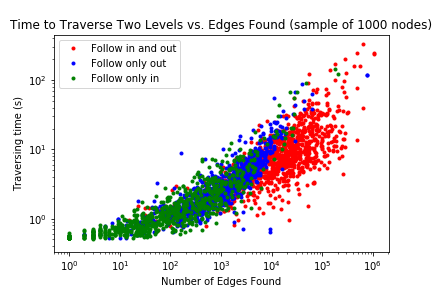
\includegraphics{./traveraltimevsedges.png}
\caption{BFS traversal times for 2 level runs showing exponential
relationship between the number of edges found and time spent
traversing}
\end{figure}

\hypertarget{mag-statistics}{%
\subsection{MAG Statistics}\label{mag-statistics}}

Using the breadth-first search tool described above, we calculated
approximate in and out degree distributions for the MAG using a random
sample of 1000 nodes.

\begin{figure}
\centering
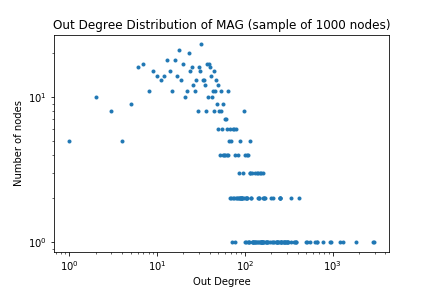
\includegraphics{./outdeg.png}
\caption{Out degree distribution of 1000 node sample of MAG made using a
one-level breadth-first search}
\end{figure}

The out degree distribution, which represents the number of referenced
papers, shows that the vast majority of papers cite under 100 papers;
however, a few cite more. This distribution does not follow the same
power law distribution commonly seen in community networks, which
intuitively makes sense given that it reflects the norms of how many
papers authors typically cite, rather than network effects.

\begin{figure}
\centering
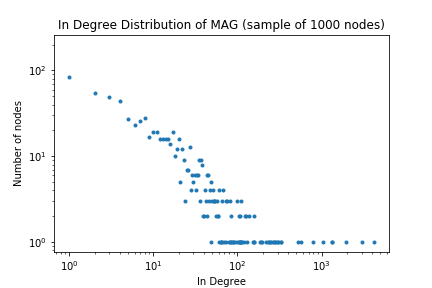
\includegraphics{./indeg.png}
\caption{In degree distribution of 1000 node sample of MAG made using a
one-level breadth-first search}
\end{figure}

The in degree distribution matches up more with a traditional power-law
network community degree distribution like that seen in web
graphs.\footnote{Broder et al., ``Graph Structure in the Web.''} This
makes intuitive sense as the mechanisms that govern who interacts with a
website by linking it and who interacts with an academic work by citing
it seem very similar.

\hypertarget{finding-development-trends-in-academic-research}{%
\section{Finding Development Trends in Academic
Research}\label{finding-development-trends-in-academic-research}}

In this paper, we evaluate various methods for reconstructing the
development of academic research. We examine methods utilizing
single-score centrality-based methods such as PageRank and node
betweenness, as well as variants of main path analysis.

\hypertarget{baselines-single-score-importance}{%
\subsection{Baselines: Single-Score
Importance}\label{baselines-single-score-importance}}

\hypertarget{pagerank}{%
\subsubsection{PageRank}\label{pagerank}}

The famous PageRank algorithm\footnote{Page et al., ``The PageRank
  Citation Ranking.''} utilizes the intuition that important nodes in a
graph are both linked to by other important nodes as well as themselves
link to other important nodes. The PageRank equation for any given node
is:

\[ r*{j} = \sum*{i \rightarrow j} \beta \frac{r_i}{d_i} + (1 - \beta) \frac{1}{n} \]

Starting from the given paper, we greedily choose the next node with the
highest PageRank score for our main path. It is worth noting that this
is not the typical use case for PageRank, which would most likely give
stronger results if it simply returned the nodes with the highest
PageRank scores in the subgraph. However, doing so would not construct a
direct lineage of research development from the source paper. In other
words, in order to compare latter main path analysis methods with our
baselines, we must compare lineages with lineages, instead of lineages
with top five raw values.

\hypertarget{node-betweenness}{%
\subsubsection{Node Betweenness}\label{node-betweenness}}

The betweenness centrality for node is the probability that a shortest
path passes through it. This measure captures the influence of a node
over the flow of information between other nodes,\footnote{Girvan and
  Newman, ``Community Structure in Social and Biological Networks.''}
and thus may prove especially fruitful for discovering the lineage of
academic knowledge. A node's betweenness centrality can be calculated
using:

\[c*{bet}(x) = \sum*{y, z \neq x, \sigma*{yz} \neq 0} \frac{\sigma*{yz}(x)}{\sigma\_{yz}}\]

where \(\sigma*{yz}\) is the number of shortest paths going from \(y\)
to \(z\), and \(\sigma*{yz}(x)\) is the number of such paths that pass
through \(x\).

Starting from the given paper, we greedily choose the next node with the
highest node betweenness centrality for our main path.

\hypertarget{main-path-analysis}{%
\subsection{Main Path Analysis}\label{main-path-analysis}}

Main path analysis is a network analysis method commonly used to find
knowledge diffusion structures in research fields through identifying a
series of connected nodes with the maximum connectivity.\footnote{Xiao
  et al., ``Knowledge Diffusion Path Analysis of Data Quality
  Literature.''} Main path analysis consists of two major algorithmic
components: computing edge traversal counts and path search.

\hypertarget{traversal-counts-search-path-count}{%
\subsubsection{Traversal Counts: Search Path
Count}\label{traversal-counts-search-path-count}}

There are many different types of edge traversal counts commonly used
with main path analysis, such as Search Path Count (SPC) and Search Path
Link Count (SPLC). Most of these types yield similar results in
practice, but previous literature suggests that search path count (SPC)
provides additional favorable properties and therefore was the most
preferred and widely used.\footnote{Xiao et al.}

Thus, we adopt SPC as our first type of traversal count. Notably, this
choice required implementing SPC from scratch in Python, as there were
no previous implementations that were easily accessible and compatible
with SNAP.

The SPC value for a given edge is the number of times it is traversed
during all possible paths from source to destination nodes. Manually
computing all possible paths in a graph is computationally expensive,
but fortunately Batagelj\footnote{Batagelj, ``Efficient Algorithms for
  Citation Network Analysis.''} devised an efficient algorithm to
compute the SPC values of all edges in \(O(\text{\# of edges})\) time.

Using the same notation as Batagelj, let \(aRb\) represents an edge from
node \(a\) to \(b\). We define two new quantities:

\[N^{-}(u) = \begin{cases}
1, & u = s \\
\sum\_{v:vRu} N^{-}(v), & \text{otherwise} \\
\end{cases} \]

Where \(N^{-}(u)\) denotes the number of paths from the source node
\(s\) to node \(u\).

\[ N^{+}(u) = \begin{cases}
1, & u = t \\
\sum\_{v:vRu} N^{+}(v), & \text{otherwise} \\
\end{cases} \]

Where \(N^{+}(u)\) denotes the number of paths from v to a destination
node \(t\) (nodes with no out-links).

\hypertarget{cycles-in-the-citation-network}{%
\subsubsection{Cycles in the Citation
Network}\label{cycles-in-the-citation-network}}

In theory, citation networks are DAGs. However, anomalies in the dataset
(i.e., revisions to papers after publishing) prevent real world citation
networks from being acyclic. This has negative consequences on SPC in
particular, which requires the graph to be acyclic.

Unfortunately, detecting and removing all cycles in a graph is extremely
expensive. To try and mitigate the effects of cycles, we create a
validation method that resolves all bidirectional edges between any pair
of nodes. To do so, we utilize MAG API requests to compare the dates of
the two nodes and remove the edge from the older paper to the newer
paper.

While this validation improves performance of SPC, it still does not
remedy the situation completely. For this reason, we turn towards a
second method of computing edge weights.

\hypertarget{traversal-counts-edge-betweenness}{%
\subsubsection{Traversal Counts: Edge
Betweenness}\label{traversal-counts-edge-betweenness}}

Edge betweenness measures the number of shortest paths passing over a
given edge in the graph. This measure specifically gives great weight to
edges that connect communities and if removed would most disrupt the
graph's underlying structure. We believe that this measure may apply
well to the case of citation networks, in which important papers can
serve as centralizing nodes that connect different subfields and related
works together. Importantly, to calculate edge betweenness we use SNAP's
built-in method that is robust to cyclic graphs.

\hypertarget{path-search}{%
\subsubsection{Path Search}\label{path-search}}

Unlike for traversal counts, different path search methods can yield
significantly different results. There are three common techniques for
constructing the main path: local search, global search and key-route
search.

For the purposes of this project, we focus on local search. Starting
from the source node (i.e., the paper under consideration), this search
greedily follows the edge with the greatest traversal count until it
reaches a destination node (i.e., a paper with no out-links in the
graph). The papers that the search encountered during its traversal make
up the main path, which are then reported as the foundational papers.

Finally, with the list of unique paper IDs identified by main path
analysis, we utilize API requests to Microsoft Academic to retrieve the
papers' titles and years. Thus, the final output of the algorithm is a
list of papers that are easily human readable and interpretable.

\hypertarget{evaluation-framework}{%
\section{Evaluation Framework}\label{evaluation-framework}}

We devised a quantitative evaluation framework that could characterize
our methods and assess their performance. To do this, we framed our
methods as a ``recommender system'' and pitted them against human and
algorithmic baselines. In pursuit of this goal, we created the following
evaluation framework:

\begin{enumerate}
\def\labelenumi{\arabic{enumi}.}
\tightlist
\item
  Choose a paper from the Microsoft Academic Graph
\item
  Manually identify the paper's top five ``most foundational papers''
\item
  Find the recommended foundational papers for each of the baselines and
  methods outlined above
\item
  Compare the recommended papers with the ground truth papers and count
  the number of matches
\end{enumerate}

We implemented this evaluation framework on three papers:

\begin{enumerate}
\def\labelenumi{\arabic{enumi}.}
\tightlist
\item
  node2vec: Scalable Feature Learning for Networks\footnote{Grover and
    Leskovec, ``Node2Vec.''}
\item
  Network Embedding as Matrix Factorization: Unifying DeepWalk, LINE,
  PTE, and node2vec\footnote{Qiu et al., ``Network Embedding as Matrix
    Factorization.''}
\item
  Values Are a Good Thing in Conservation Biology\footnote{Noss,
    ``Values Are a Good Thing in Conservation Biology.''}
\end{enumerate}

In manually identifying papers, however, we realized the difficulty of
the task for a non-expert non-author person to identify lineages or
foundational papers. A key aspect of lineages and foundational papers is
that they need not be direct citations and also depend heavily on their
location within the academic graph. If we find a paper that is both
cited cited by every other direct citation of another paper, that paper
is likely very foundational, but it is exceedingly difficult for a
non-expert reader to identify. We have ideas for how to better frame
quantitative analysis of such methods that we discuss in our future work
section.

Thus, we decided to reframe our evaluation as qualitative and focus it
on identifying key characteristics between different methods and
parameters. This analysis must be qualitative because it is hard to
define exactly what lineages are and what results are ``good''. We focus
more on what our methods are doing and what properties of the citation
network they seem to be highlighting.

\hypertarget{results}{%
\section{Results}\label{results}}

The following tables show the results of running the evaluation
framework on the three aforementioned papers for BFS graphs of 2 levels
following only out-links, 2 levels following both out- and in-links, and
3 levels following only out-links were computed.

\begin{longtable}[]{@{}ccccc@{}}
\toprule
BFS Parameters & MPA (SPC) & MPA (Edge Betweenness) & PageRank & Node
Betweenness\tabularnewline
\midrule
\endhead
2 levels, out-links & 2 & 0 & 0 & 1\tabularnewline
2 levels, out- and in-links & 1 & 0 & 0 & 0\tabularnewline
3 levels, out-links & 0 & 0 & 0 & 0\tabularnewline
\bottomrule
\end{longtable}

\begin{longtable}[]{@{}ccccc@{}}
\toprule
BFS Parameters & MPA (SPC) & MPA (Edge Betweenness) & PageRank & Node
Betweenness\tabularnewline
\midrule
\endhead
2 levels, out-links & 2 & 0 & 1 & 1\tabularnewline
2 levels, out- and in-links & 3 & 0 & 0 & 0\tabularnewline
3 levels, out-links & 0 & 0 & 0 & 0\tabularnewline
\bottomrule
\end{longtable}

\begin{longtable}[]{@{}ccccc@{}}
\toprule
BFS Parameters & MPA (SPC) & MPA (Edge Betweenness) & PageRank & Node
Betweenness\tabularnewline
\midrule
\endhead
2 levels, out-links & 2 & 1 & 1 & 1\tabularnewline
2 levels, out- and in-links & 1 & 2 & 0 & 1\tabularnewline
3 levels, out-links & 1 & 2 & 0 & 1\tabularnewline
\bottomrule
\end{longtable}

\begin{longtable}[]{@{}ccccc@{}}
\toprule
Method & MPA (SPC) & MPA (Edge Betweenness) & PageRank & Node
Betweenness\tabularnewline
\midrule
\endhead
Total \# Matches & 9 & 5 & 2 & 5\tabularnewline
\% of Total Matches & 42.9\% & 23.8\% & 9.5\% & 23.8\%\tabularnewline
\bottomrule
\end{longtable}

\begin{longtable}[]{@{}ccc@{}}
\toprule
BFS Parameters & Total \# Matches & \% of Total Matches\tabularnewline
\midrule
\endhead
2 levels, out-links & 12 & 50.0\%\tabularnewline
2 levels, out- and in-links & 8 & 33.3\%\tabularnewline
3 levels, out-links & 4 & 16.7\%\tabularnewline
\bottomrule
\end{longtable}

We have also listed each method's specific recommendations for each of
the three aforementioned papers in the attached appendix.

\hypertarget{discussion}{%
\section{Discussion}\label{discussion}}

Looking at the quantitative results, we notice two distinct trends
emerge from the data. First, the BFS graph for 2 levels following only
out-links has the highest number of total matches for all three papers.
We believe this may be due in part to the fact that shorter hop BFS
graphs capture more accurately paper-specific neighborhoods, thus
emphasizing papers that are of high importance in relation to the source
paper.

However, we also acknowledge that this result may be due to a faulty
evaluation method. When curating the ``ground truth'' foundational
papers for the three papers in the test set, there is most likely a
strong bias towards choosing papers that appear in the given paper's
direct references, as those will be the papers whose ideas are most
strongly cited on first read. Thus, the chosen ground truth papers are
more biased towards a paper's direct references rather than its
indirect, transitive references, which will serve to bias the methods'
performance to the smaller BFS subgraphs. We will discuss improvements
to the evaluation method in the future work section.

Secondly, MPA using SPC achieves the highest number of total matches
across all three papers with 9 total matches. This result is promising,
even when using a non-robust evaluation metric, and can also be
corroborated by the qualitative results (see Appendix). For example, for
the paper ``Network Embedding as Matrix Factorization: Unifying
DeepWalk, LINE, PTE, and node2vec'' (Qiu et al., 2018) using the BFS
subgraph on two levels following only out-links, the main path
constructing using SPC traversal counts captures three of the methods
mentioned in the paper title. It further includes papers on
representation learning and dimensionality reduction, which are both
foundational concepts utilized in the paper. Similar qualitative
analysis of the other BFS subgraphs of two levels following only
out-links produces similarly strong results.

In comparison, choosing nodes on the main path based on highest PageRank
scores performs the worst. This result can be explained in one part by
the unconventional use of PageRank in choosing the next node for the
main path, as well as by the BFS subgraph sometimes only being
constructed on out-links. Furthermore, taking a qualitative look at the
PageRank results, it is often derailed from the intuitive ``main path''
by picking papers that have high importance but are so far removed from
the given paper that the link between the two can be hard to interpret.
One can see this quantitatively by the fact that the PageRank paths are
on average shorter than the paths produced by other methods.

It is worth noting, however, that almost all the methods do not perform
as well when used on larger BFS subgraphs or BFS subgraphs that follow
in-links. In particular, following in-links proves a difficult challenge
as it only requires a few popular papers with hundreds or even thousands
of citations to blow up the BFS subgraph dramatically. It was for this
reason that a BFS subgraph of three levels following both in- and
out-links was not feasible for this paper, as while we could extract the
subgraphs successfully (which generally had around 1.5 million to 3
million nodes), the methods would take enormous amounts of time to
complete.

Overall, while the results are not definitive in proving that MPA is
strictly better than any existing methods, preliminary quantitative and
qualitative analysis of the produced paths provides evidence for the
potential of MPA using SPC and node betweenness in constructing
development trends of academic research. In particular, we show that MPA
offers information that is different and complementary to that
traditionally provided by citation recommendation systems through its
creation of lineages of connected academic works specific to the given
paper rather than collections of generally important works in a field.

Furthermore, our paper contributes a novel application of MPA to the
MAG, which offers a promise for identifying structures of academia for
any field or concept contained in the dataset. Ultimately, we hope to
provide one small step forward in the pursuit of increasing
accessibility to research and academia for all.

\hypertarget{future-work}{%
\section{Future Work}\label{future-work}}

As mentioned above, quantitative evaluation of any methods designed to
understand the foundations and lineages of papers must find some
representation of a ground truth. However, such ground truth measures
are difficult for non-experts to formulate and even define. We believe
that there is room for an empirical study to help determine what the
ground truth development structures are for certain papers, which would
necessitate going to domain experts and surveying them to hear their
ideas of what influence a given paper the most.

We anticipate that actually defining ``foundational'' papers and
``lineages'' of papers in a consistently-interpreted way will be a
challenge. Any study would need to address these vague concepts with
clear definitions that could be interpreted in the same manner by the
authors surveyed. A study like this would allow for some ground-truth
data on what our algorithms should be looking for when we seek to
identify foundational papers.

This project is also meant as a starting point for studies of
interdisciplinary academic structure that require working with a
comprehensive citation network. This opens the door for research that
seeks to determine to what extent do different disciplines interact with
each other and identify ``filter-bubbles'' where different disciplines
might argue over the same concept without ever interacting with the
literature, and academic lineages, of their opponents.

Finally, there remains much potential for improvement of the methods
used in this paper. For example, adapting SPC to handle cyclic graphs or
applying an efficient method for removing cycles may boost its
performance. Additionally, MPA using SPC and edge betweenness tends to
produce main paths of long lengths, and thus discouraging this behavior
using damping or weighting nodes by their marginal gain (i.e., the
number of unique papers they add in a set cover) may help with
condensing the results.

\hypertarget{references}{%
\section{References}\label{references}}

\hypertarget{refs}{}
\leavevmode\hypertarget{ref-batageljEfficientAlgorithmsCitation2003}{}%
Batagelj, Vladimir. ``Efficient Algorithms for Citation Network
Analysis,'' September 13, 2003. \url{http://arxiv.org/abs/cs/0309023}.

\leavevmode\hypertarget{ref-bergstromEigenfactorMetrics2008}{}%
Bergstrom, Carl T., Jevin D. West, and Marc A. Wiseman. ``The
Eigenfactor™ Metrics.'' \emph{Journal of Neuroscience} 28, no. 45
(November 5, 2008): 11433--4.
\url{https://doi.org/10.1523/JNEUROSCI.0003-08.2008}.

\leavevmode\hypertarget{ref-broderGraphStructureWeb2000}{}%
Broder, Andrei, Ravi Kumar, Farzin Maghoul, Prabhakar Raghavan, Sridhar
Rajagopalan, Raymie Stata, Andrew Tomkins, and Janet Wiener. ``Graph
Structure in the Web.'' \emph{Computer Networks}, 2000, 12.

\leavevmode\hypertarget{ref-calero-medinaCombiningMappingCitation2008}{}%
Calero-Medina, Clara, and Ed C. M. Noyons. ``Combining Mapping and
Citation Network Analysis for a Better Understanding of the Scientific
Development: The Case of the Absorptive Capacity Field.'' \emph{Journal
of Informetrics} 2, no. 4 (October 1, 2008): 272--79.
\url{https://doi.org/10.1016/j.joi.2008.09.005}.

\leavevmode\hypertarget{ref-girvanCommunityStructureSocial2002}{}%
Girvan, M., and M. E. J. Newman. ``Community Structure in Social and
Biological Networks.'' \emph{Proceedings of the National Academy of
Sciences} 99, no. 12 (June 11, 2002): 7821--6.
\url{https://doi.org/10.1073/pnas.122653799}.

\leavevmode\hypertarget{ref-groverNode2VecScalableFeature2016}{}%
Grover, Aditya, and Jure Leskovec. ``Node2Vec: Scalable Feature Learning
for Networks.'' In \emph{Proceedings of the 22Nd ACM SIGKDD
International Conference on Knowledge Discovery and Data Mining},
855--64. KDD '16. New York, NY, USA: ACM, 2016.
\url{https://doi.org/10.1145/2939672.2939754}.

\leavevmode\hypertarget{ref-herrmannovaAnalysisMicrosoftAcademic2016}{}%
Herrmannova, Drahomira, and Petr Knoth. ``An Analysis of the Microsoft
Academic Graph.'' \emph{D-Lib Magazine} 22, no. 9/10 (September 2016).
\url{https://doi.org/10.1045/september2016-herrmannova}.

\leavevmode\hypertarget{ref-ImpactFactorClarivate}{}%
``Impact Factor - Clarivate.'' Accessed October 18, 2018.
\url{https://clarivate.com/essays/impact-factor/}.

\leavevmode\hypertarget{ref-kyrolaGraphChiLargeScaleGraph}{}%
Kyrola, Aapo, Guy Blelloch, and Carlos Guestrin. ``GraphChi: Large-Scale
Graph Computation on Just a PC,'' n.d., 16.

\leavevmode\hypertarget{ref-liuIntegratedApproachMain2012}{}%
Liu, John S., and Louis Y. Y. Lu. ``An Integrated Approach for Main Path
Analysis: Development of the Hirsch Index as an Example.'' \emph{Journal
of the American Society for Information Science and Technology} 63, no.
3 (March 1, 2012): 528--42. \url{https://doi.org/10.1002/asi.21692}.

\leavevmode\hypertarget{ref-nossValuesAreGood2007a}{}%
Noss, Reed F. ``Values Are a Good Thing in Conservation Biology.''
\emph{Conservation Biology} 21, no. 1 (February 1, 2007): 18--20.
\url{https://doi.org/10.1111/j.1523-1739.2006.00637.x}.

\leavevmode\hypertarget{ref-pagePageRankCitationRanking1998}{}%
Page, Larry, Sergey Brin, R. Motwani, and T. Winograd. ``The PageRank
Citation Ranking: Bringing Order to the Web,'' 1998.

\leavevmode\hypertarget{ref-qiuNetworkEmbeddingMatrix2018}{}%
Qiu, Jiezhong, Yuxiao Dong, Hao Ma, Jian Li, Kuansan Wang, and Jie Tang.
``Network Embedding as Matrix Factorization: Unifying DeepWalk, LINE,
PTE, and Node2vec.'' \emph{Proceedings of the Eleventh ACM International
Conference on Web Search and Data Mining - WSDM '18}, 2018, 459--67.
\url{https://doi.org/10.1145/3159652.3159706}.

\leavevmode\hypertarget{ref-royXStreamEdgecentricGraph2013}{}%
Roy, Amitabha, Ivo Mihailovic, and Willy Zwaenepoel. ``X-Stream:
Edge-Centric Graph Processing Using Streaming Partitions.'' In
\emph{Proceedings of the Twenty-Fourth ACM Symposium on Operating
Systems Principles - SOSP '13}, 472--88. Farminton, Pennsylvania: ACM
Press, 2013. \url{https://doi.org/10.1145/2517349.2522740}.

\leavevmode\hypertarget{ref-sinhaOverviewMicrosoftAcademic2015}{}%
Sinha, Arnab, Zhihong Shen, Yang Song, Hao Ma, Darrin Eide, Bo-June
(Paul) Hsu, and Kuansan Wang. ``An Overview of Microsoft Academic
Service (MAS) and Applications.'' In \emph{Proceedings of the 24th
International Conference on World Wide Web - WWW '15 Companion},
243--46. Florence, Italy: ACM Press, 2015.
\url{https://doi.org/10.1145/2740908.2742839}.

\leavevmode\hypertarget{ref-OppositeBloomFilter2012}{}%
``The Opposite of a Bloom Filter -- Something Similar,'' May 21, 2012.
\url{https://www.somethingsimilar.com/2012/05/21/the-opposite-of-a-bloom-filter/}.

\leavevmode\hypertarget{ref-treatProbabilisticDataStructures2018}{}%
Treat, Tyler. \emph{Probabilistic Data Structures for Processing
Continuous, Unbounded Streams.: Tylertreat/BoomFilters}, 2018.
\url{https://github.com/tylertreat/BoomFilters}.

\leavevmode\hypertarget{ref-xiaoKnowledgeDiffusionPath2014}{}%
Xiao, Yu, Louis Y. Y. Lu, John S. Liu, and Zhili Zhou. ``Knowledge
Diffusion Path Analysis of Data Quality Literature: A Main Path
Analysis.'' \emph{Journal of Informetrics} 8, no. 3 (July 1, 2014):
594--605. \url{https://doi.org/10.1016/j.joi.2014.05.001}.

\hypertarget{appendix}{%
\section{Appendix}\label{appendix}}

This appendix contains the results from constructing paths of academic
research from the three papers mentioned in the paper. The four methods
utilized were MPA using SPC, MPA using edge betweenness, PageRank, and
node betweenness.

Sometimes, the maximum value for the weight of an edge or nodes is 0, in
which case the next node in the path is chosen arbitrarily from all the
neighbors of the previous node. This case results from failing due to
cycles in the graph (i.e., MPA using SPC) or other anomalies. These
edges/nodes are denoted in the results with an *.

\hypertarget{node2vec-scalable-feature-learning-for-networks-grover-leskovec-2016}{%
\subsection{node2vec: Scalable Feature Learning for Networks (Grover \&
Leskovec,
2016)}\label{node2vec-scalable-feature-learning-for-networks-grover-leskovec-2016}}

\hypertarget{bfs-graph-1395-nodes-1684-edges-2-levels-following-only-out-links}{%
\subsubsection{BFS Graph (1395 nodes, 1684 edges): 2 levels, following
only
out-links}\label{bfs-graph-1395-nodes-1684-edges-2-levels-following-only-out-links}}

\hypertarget{main-path-analyis-spc}{%
\paragraph{Main Path Analyis (SPC)}\label{main-path-analyis-spc}}

\begin{enumerate}
\def\labelenumi{\arabic{enumi}.}
\tightlist
\item
  grarep learning graph representations with global structural
  information (2015)
\item
  line large scale information network embedding (2015)
\item
  deepwalk online learning of social representations (2014)
\item
  representation learning a review and new perspectives (2013)
\item
  a global geometric framework for nonlinear dimensionality reduction
  (2000)
\item
  image representations for visual learning (1996)
\end{enumerate}

\hypertarget{main-path-analyis-edge-betweenness}{%
\paragraph{Main Path Analyis (Edge
Betweenness)}\label{main-path-analyis-edge-betweenness}}

\begin{enumerate}
\def\labelenumi{\arabic{enumi}.}
\tightlist
\item
  community detection in graphs (2010)
\item
  chemical oscillations waves and turbulence (1984)
\end{enumerate}

\hypertarget{pagerank-1}{%
\paragraph{PageRank}\label{pagerank-1}}

\begin{enumerate}
\def\labelenumi{\arabic{enumi}.}
\tightlist
\item
  nonlinear dimensionality reduction by locally linear embedding (2000)
\item
  learning the parts of objects by non negative matrix factorization
  (1999)
\end{enumerate}

\hypertarget{node-betweeness}{%
\paragraph{Node Betweeness}\label{node-betweeness}}

\begin{enumerate}
\def\labelenumi{\arabic{enumi}.}
\tightlist
\item
  deepwalk online learning of social representations (2014)
\item
  representation learning a review and new perspectives (2013)
\item
  a global geometric framework for nonlinear dimensionality reduction
  (2000)
\item
  independent component analysis a new concept (1994)*
\end{enumerate}

\hypertarget{bfs-graph-1395-nodes-1684-edges-2-levels-following-only-out-links-1}{%
\subsubsection{BFS Graph (1395 nodes, 1684 edges): 2 levels, following
only
out-links}\label{bfs-graph-1395-nodes-1684-edges-2-levels-following-only-out-links-1}}

\hypertarget{main-path-analyis-spc-1}{%
\paragraph{Main Path Analyis (SPC)}\label{main-path-analyis-spc-1}}

\begin{enumerate}
\def\labelenumi{\arabic{enumi}.}
\tightlist
\item
  community detection in graphs (2010)*
\item
  random walks markov processes and the multiscale modular organization
  of complex networks (2014)*
\end{enumerate}

\hypertarget{main-path-analyis-edge-betweenness-1}{%
\paragraph{Main Path Analyis (Edge
Betweenness)}\label{main-path-analyis-edge-betweenness-1}}

\begin{enumerate}
\def\labelenumi{\arabic{enumi}.}
\tightlist
\item
  community detection in graphs (2010)
\item
  the principal components analysis of a graph and its relationships to
  spectral clustering (2004)
\item
  laplacian eigenmaps and spectral techniques for embedding and
  clustering (2001)
\item
  a global geometric framework for nonlinear dimensionality reduction
  (2000)
\item
  perceptual cognitive universals as reflections of the world (1994)
\end{enumerate}

\hypertarget{pagerank-2}{%
\paragraph{PageRank}\label{pagerank-2}}

\begin{enumerate}
\def\labelenumi{\arabic{enumi}.}
\tightlist
\item
  nonlinear dimensionality reduction by locally linear embedding (2000)
\item
  image representations for visual learning (1996)
\end{enumerate}

\hypertarget{node-betweeness-1}{%
\paragraph{Node Betweeness}\label{node-betweeness-1}}

\begin{enumerate}
\def\labelenumi{\arabic{enumi}.}
\tightlist
\item
  community detection in graphs (2010)
\item
  random walk computation of similarities between nodes of a graph with
  application to collaborative recommendation (2007)
\item
  laplacian eigenmaps and spectral techniques for embedding and
  clustering (2001)
\item
  normalized cuts and image segmentation (2000)*
\end{enumerate}

\hypertarget{bfs-graph-19854-nodes-38148-edges-3-levels-following-only-out-links}{%
\subsubsection{BFS Graph (19854 nodes, 38148 edges): 3 levels, following
only
out-links}\label{bfs-graph-19854-nodes-38148-edges-3-levels-following-only-out-links}}

\hypertarget{main-path-analysis-spc}{%
\paragraph{Main Path Analysis (SPC)}\label{main-path-analysis-spc}}

\begin{enumerate}
\def\labelenumi{\arabic{enumi}.}
\tightlist
\item
  a large scale evaluation of computational protein function prediction
  (2013)
\item
  analysis of protein function and its prediction from amino acid
  sequence (2011)
\item
  annotation error in public databases misannotation of molecular
  function in enzyme superfamilies (2009)
\item
  protein function prediction the power of multiplicity (2009)
\item
  network based prediction of protein function (2007)
\item
  cfinder locating cliques and overlapping modules in biological
  networks (2006)
\item
  cytoscape a software environment for integrated models of biomolecular
  interaction networks (2003)*
\end{enumerate}

\hypertarget{main-path-analysis-edge-betweenness}{%
\paragraph{Main Path Analysis (Edge
Betweenness)}\label{main-path-analysis-edge-betweenness}}

\begin{enumerate}
\def\labelenumi{\arabic{enumi}.}
\tightlist
\item
  community detection in graphs (2010)
\item
  microscopic evolution of social networks (2008)
\item
  relational learning via latent social dimensions (2009)
\item
  using ghost edges for classification in sparsely labeled networks
  (2008)
\item
  semi supervised learning literature survey (2006)
\item
  self taught learning transfer learning from unlabeled data (2007)
\item
  reducing the dimensionality of data with neural networks (2006)
\item
  a fast learning algorithm for deep belief nets (2006)
\item
  justifying and generalizing contrastive divergence (2009)
\item
  semantic hashing (2009)
\item
  rcv1 a new benchmark collection for text categorization research
  (2004)
\item
  machine learning in automated text categorization (2002)
\item
  enhanced hypertext categorization using hyperlinks (1998)
\item
  on the foundations of relaxation labeling processes (1987)
\item
  relaxation and constrained optimization by local processes (1979)
\end{enumerate}

\hypertarget{pagerank-3}{%
\paragraph{PageRank}\label{pagerank-3}}

\begin{enumerate}
\def\labelenumi{\arabic{enumi}.}
\tightlist
\item
  nonlinear dimensionality reduction by locally linear embedding (2000)
\item
  dimension reduction by local principal component analysis (1997)
\item
  replicator neural networks for universal optimal source coding (1995)
\item
  the wake sleep algorithm for unsupervised neural networks (1995)
\end{enumerate}

\hypertarget{node-betweeness-2}{%
\paragraph{Node Betweeness}\label{node-betweeness-2}}

\begin{enumerate}
\def\labelenumi{\arabic{enumi}.}
\tightlist
\item
  community detection in graphs (2010)
\item
  the structure and function of complex networks (2003)
\item
  statistical mechanics of complex networks (2001)
\item
  clustering and preferential attachment in growing networks (2001)
\item
  the structure of scientific collaboration networks (2001)
\item
  structural cohesion and embeddedness a hierarchical concept of social
  groups (2003)
\item
  models of core periphery structures (2000)
\item
  optimization by simulated annealing (1983)
\item
  solvable model of a spin glass (1975)
\item
  photon cross sections attenuation coefficients and energy absorption
  coefficients from 10 kev to 100 gev (1969)*
\end{enumerate}

\hypertarget{network-embedding-as-matrix-factorization-unifying-deepwalk-line-pte-and-node2vec-qiu-et-al.-2018}{%
\subsection{Network Embedding as Matrix Factorization: Unifying
DeepWalk, LINE, PTE, and node2vec (Qiu et al.,
2018)}\label{network-embedding-as-matrix-factorization-unifying-deepwalk-line-pte-and-node2vec-qiu-et-al.-2018}}

\hypertarget{bfs-graph-1155-nodes-1571-edges-2-levels-following-only-out-links}{%
\subsubsection{BFS Graph (1155 nodes, 1571 edges): 2 levels, following
only
out-links}\label{bfs-graph-1155-nodes-1571-edges-2-levels-following-only-out-links}}

\hypertarget{main-path-analysis-spc-1}{%
\paragraph{Main Path Analysis (SPC)}\label{main-path-analysis-spc-1}}

\begin{enumerate}
\def\labelenumi{\arabic{enumi}.}
\tightlist
\item
  network embedding as matrix factorization unifying deepwalk line pte
  and node2vec (2018)
\item
  inductive representation learning on large graphs (2017)
\item
  structural deep network embedding (2016)
\item
  grarep learning graph representations with global structural
  information (2015)
\item
  line large scale information network embedding (2015)
\item
  deepwalk online learning of social representations (2014)
\item
  representation learning a review and new perspectives (2013)
\item
  nonlinear dimensionality reduction by locally linear embedding (2000)
\end{enumerate}

\hypertarget{main-path-analysis-edge-betweenness-1}{%
\paragraph{Main Path Analysis (Edge
Betweenness)}\label{main-path-analysis-edge-betweenness-1}}

\begin{enumerate}
\def\labelenumi{\arabic{enumi}.}
\tightlist
\item
  network embedding as matrix factorization unifying deepwalk line pte
  and node2vec (2018)
\item
  representation learning a review and new perspectives (2013)
\item
  modeling pixel means and covariances using factorized third order
  boltzmann machines (2010)
\end{enumerate}

\hypertarget{pagerank-4}{%
\paragraph{PageRank}\label{pagerank-4}}

\begin{enumerate}
\def\labelenumi{\arabic{enumi}.}
\tightlist
\item
  network embedding as matrix factorization unifying deepwalk line pte
  and node2vec (2018)
\item
  deepwalk online learning of social representations (2014)
\item
  efficient estimation of word representations in vector space (2013)
\item
  linguistic regularities in continuous space word representations
  (2013)
\end{enumerate}

\hypertarget{node-betweenness-1}{%
\paragraph{Node Betweenness}\label{node-betweenness-1}}

\begin{enumerate}
\def\labelenumi{\arabic{enumi}.}
\tightlist
\item
  network embedding as matrix factorization unifying deepwalk line pte
  and node2vec (2018)
\item
  deepwalk online learning of social representations (2014)
\item
  representation learning a review and new perspectives (2013)
\item
  imagenet classification with deep convolutional neural networks
  (2012)*
\end{enumerate}

\hypertarget{bfs-graph-47035-nodes-55686-edges-2-levels-following-both-out-links-and-in-links}{%
\subsubsection{BFS Graph (47035 nodes, 55686 edges): 2 levels, following
both out-links and
in-links}\label{bfs-graph-47035-nodes-55686-edges-2-levels-following-both-out-links-and-in-links}}

\hypertarget{main-path-analysis-spc-2}{%
\paragraph{Main Path Analysis (SPC)}\label{main-path-analysis-spc-2}}

\begin{enumerate}
\def\labelenumi{\arabic{enumi}.}
\tightlist
\item
  network embedding as matrix factorization unifying deepwalk line pte
  and node2vec (2018)
\item
  inductive representation learning on large graphs (2017)
\item
  community preserving network embedding (2017)
\item
  node2vec scalable feature learning for networks (2016)
\item
  grarep learning graph representations with global structural
  information (2015)
\item
  line large scale information network embedding (2015)
\item
  deepwalk online learning of social representations (2014)
\item
  leveraging social media networks for classification (2011)
\item
  empirical comparison of algorithms for network community detection
  (2010)
\item
  community detection in graphs (2010)
\item
  a tutorial on spectral clustering (2007)
\item
  random walk computation of similarities between nodes of a graph with
  application to collaborative recommendation (2007)
\item
  normalized cuts and image segmentation (2000)
\item
  spectral graph theory (1996)
\item
  asymptotic analysis of a random walk on a hypercube with many
  dimensions (1990)
\end{enumerate}

\hypertarget{main-path-analysis-edge-betweenness-2}{%
\paragraph{Main Path Analysis (Edge
Betweenness)}\label{main-path-analysis-edge-betweenness-2}}

\begin{enumerate}
\def\labelenumi{\arabic{enumi}.}
\tightlist
\item
  network embedding as matrix factorization unifying deepwalk line pte
  and node2vec (2018)
\item
  mining multi label data (2009)
\item
  hypergraph spectral learning for multi label classification (2008)
\item
  spectral graph theory (1996)
\item
  asymptotic analysis of a random walk on a hypercube with many
  dimensions (1990)
\end{enumerate}

\hypertarget{pagerank-5}{%
\paragraph{PageRank}\label{pagerank-5}}

\begin{enumerate}
\def\labelenumi{\arabic{enumi}.}
\tightlist
\item
  network embedding as matrix factorization unifying deepwalk line pte
  and node2vec (2018)
\item
  normalized cuts and image segmentation (2000)
\item
  spectral graph theory (1996)
\item
  asymptotic analysis of a random walk on a hypercube with many
  dimensions (1990)
\end{enumerate}

\hypertarget{node-betweenness-2}{%
\paragraph{Node Betweenness}\label{node-betweenness-2}}

\begin{enumerate}
\def\labelenumi{\arabic{enumi}.}
\tightlist
\item
  network embedding as matrix factorization unifying deepwalk line pte
  and node2vec (2018)
\item
  representation learning a review and new perspectives (2013)
\item
  natural language processing almost from scratch (2011)
\item
  feature rich part of speech tagging with a cyclic dependency network
  (2003)
\item
  text categorization based on regularized linear classification methods
  (2001)*
\end{enumerate}

\hypertarget{bfs-graph-17866-nodes-34040-edges-3-levels-following-only-out-links}{%
\subsubsection{BFS Graph (17866 nodes, 34040 edges): 3 levels, following
only
out-links}\label{bfs-graph-17866-nodes-34040-edges-3-levels-following-only-out-links}}

\hypertarget{main-path-analysis-spc-3}{%
\paragraph{Main Path Analysis (SPC)}\label{main-path-analysis-spc-3}}

\begin{enumerate}
\def\labelenumi{\arabic{enumi}.}
\tightlist
\item
  network embedding as matrix factorization unifying deepwalk line pte
  and node2vec (2018)
\item
  a unifying theorem for spectral embedding and clustering (2003)
\item
  nonlinear component analysis as a kernel eigenvalue problem (1998)*
\item
  support vector networks (1995)*
\end{enumerate}

\hypertarget{main-path-analysis-edge-betweenness-3}{%
\paragraph{Main Path Analysis (Edge
Betweenness)}\label{main-path-analysis-edge-betweenness-3}}

\begin{enumerate}
\def\labelenumi{\arabic{enumi}.}
\tightlist
\item
  network embedding as matrix factorization unifying deepwalk line pte
  and node2vec (2018)
\item
  representation learning a review and new perspectives (2013)
\item
  bayesian and l1 approaches to sparse unsupervised learning (2011)
\item
  mixed membership stochastic blockmodels (2008)
\item
  model based clustering for social networks (2007)
\item
  bayesian cluster analysis (1978)
\end{enumerate}

\hypertarget{pagerank-6}{%
\paragraph{PageRank}\label{pagerank-6}}

\begin{enumerate}
\def\labelenumi{\arabic{enumi}.}
\tightlist
\item
  network embedding as matrix factorization unifying deepwalk line pte
  and node2vec (2018)
\item
  spectral graph theory (1996)
\item
  spectra of graphs (1980)
\item
  algebraic connectivity of graphs (1973)
\end{enumerate}

\hypertarget{node-betweenness-3}{%
\paragraph{Node Betweenness}\label{node-betweenness-3}}

\begin{enumerate}
\def\labelenumi{\arabic{enumi}.}
\tightlist
\item
  network embedding as matrix factorization unifying deepwalk line pte
  and node2vec (2018)
\item
  representation learning a review and new perspectives (2013)
\item
  learning deep architectures for ai (2009)
\item
  a fast learning algorithm for deep belief nets (2006)
\item
  justifying and generalizing contrastive divergence (2009)
\item
  scaling learning algorithms towards ai (2007)
\item
  semi supervised learning using gaussian fields and harmonic functions
  (2003)
\item
  normalized cuts and image segmentation (2000)
\item
  spectral graph theory (1996)
\item
  spectra of graphs (1980)
\item
  matrix iterative analysis (1962)*
\end{enumerate}

\hypertarget{values-are-a-good-thing-in-conservation-biology-noss-2007}{%
\subsection{Values are a Good Thing in Conservation Biology (Noss,
2007)}\label{values-are-a-good-thing-in-conservation-biology-noss-2007}}

\hypertarget{bfs-graph-164-nodes-171-edges-2-levels-following-only-out-links}{%
\subsubsection{BFS Graph (164 nodes, 171 edges): 2 levels, following
only
out-links}\label{bfs-graph-164-nodes-171-edges-2-levels-following-only-out-links}}

\hypertarget{main-path-analysis-spc-4}{%
\paragraph{Main Path Analysis (SPC)}\label{main-path-analysis-spc-4}}

\begin{enumerate}
\def\labelenumi{\arabic{enumi}.}
\tightlist
\item
  values are a good thing in conservation biology (2007)
\item
  ecology values and objectivity advancing the debate (2005)
\item
  beyond biology toward a more public ecology for conservation (2001)
\item
  method in ecology strategies for conservation (1993)
\end{enumerate}

\hypertarget{main-path-analysis-edge-betweenness-4}{%
\paragraph{Main Path Analysis (Edge
Betweenness)}\label{main-path-analysis-edge-betweenness-4}}

\begin{enumerate}
\def\labelenumi{\arabic{enumi}.}
\tightlist
\item
  values are a good thing in conservation biology (2007)
\item
  beyond biology toward a more public ecology for conservation (2001)
\item
  cultural sustainability aligning aesthetics and ecology (1997)
\end{enumerate}

\hypertarget{pagerank-7}{%
\paragraph{PageRank}\label{pagerank-7}}

\begin{enumerate}
\def\labelenumi{\arabic{enumi}.}
\tightlist
\item
  values are a good thing in conservation biology (2007)
\item
  advocacy and credibility of ecological scientists in resource
  decision-making a regional study (2003)
\item
  entering the century of the environment a new social contract for
  science (1998)
\end{enumerate}

\hypertarget{node-betweenness-4}{%
\paragraph{Node Betweenness}\label{node-betweenness-4}}

\begin{enumerate}
\def\labelenumi{\arabic{enumi}.}
\tightlist
\item
  values are a good thing in conservation biology (2007)
\item
  beyond biology toward a more public ecology for conservation (2001)
\item
  compass and gyroscope integrating science and politics for the
  environment (1993)*
\end{enumerate}

\hypertarget{bfs-graph-5696-nodes-6430-edges-2-levels-following-both-out-links-and-in-links}{%
\subsubsection{BFS Graph (5696 nodes, 6430 edges): 2 levels, following
both out-links and
in-links}\label{bfs-graph-5696-nodes-6430-edges-2-levels-following-both-out-links-and-in-links}}

\hypertarget{main-path-analysis-spc-5}{%
\paragraph{Main Path Analysis (SPC)}\label{main-path-analysis-spc-5}}

\begin{enumerate}
\def\labelenumi{\arabic{enumi}.}
\tightlist
\item
  values are a good thing in conservation biology (2007)
\item
  ecology values and objectivity advancing the debate (2005)
\item
  beyond biology toward a more public ecology for conservation (2001)
\item
  a science for survival values and conservation biology (1996)
\item
  a sand county almanac (1949)
\end{enumerate}

\hypertarget{main-path-analysis-edge-betweenness-5}{%
\paragraph{Main Path Analysis (Edge
Betweenness)}\label{main-path-analysis-edge-betweenness-5}}

\begin{enumerate}
\def\labelenumi{\arabic{enumi}.}
\tightlist
\item
  values are a good thing in conservation biology (2007)
\item
  beyond biology toward a more public ecology for conservation (2001)
\item
  the appearance of ecological systems as a matter of policy (1992)
\item
  a sand county almanac (1949)
\end{enumerate}

\hypertarget{pagerank-8}{%
\paragraph{PageRank}\label{pagerank-8}}

\begin{enumerate}
\def\labelenumi{\arabic{enumi}.}
\tightlist
\item
  values are a good thing in conservation biology (2007)
\item
  a sand county almanac (1949)
\end{enumerate}

\hypertarget{node-betweenness-5}{%
\paragraph{Node Betweenness}\label{node-betweenness-5}}

\begin{enumerate}
\def\labelenumi{\arabic{enumi}.}
\tightlist
\item
  values are a good thing in conservation biology (2007)
\item
  beyond biology toward a more public ecology for conservation (2001)
\item
  a science for survival values and conservation biology (1996)
\item
  the obligations of a biologist (1989)*
\end{enumerate}

\hypertarget{bfs-graph-3065-nodes-3460-edges-3-levels-following-only-out-links}{%
\subsubsection{BFS Graph (3065 nodes, 3460 edges): 3 levels, following
only
out-links}\label{bfs-graph-3065-nodes-3460-edges-3-levels-following-only-out-links}}

\hypertarget{main-path-analysis-spc-6}{%
\paragraph{Main Path Analysis (SPC)}\label{main-path-analysis-spc-6}}

\begin{enumerate}
\def\labelenumi{\arabic{enumi}.}
\tightlist
\item
  values are a good thing in conservation biology (2007)
\item
  ecology values and objectivity advancing the debate (2005)
\item
  implications of current ecological thinking for biodiversity
  conservation a review of the salient issues (2005)
\item
  beyond biology toward a more public ecology for conservation (2001)
\item
  the natural imperative for biological conservation (2000)
\item
  current normative concepts in conservation (1999)
\item
  cross scale morphology geometry and dynamics of ecosystems (1992)
\item
  large scale management experiments and learning by doing (1990)
\item
  adaptive environmental assessment and management (1978)
\end{enumerate}

\hypertarget{main-path-analysis-edge-betweenness-6}{%
\paragraph{Main Path Analysis (Edge
Betweenness)}\label{main-path-analysis-edge-betweenness-6}}

\begin{enumerate}
\def\labelenumi{\arabic{enumi}.}
\tightlist
\item
  values are a good thing in conservation biology (2007)
\item
  beyond biology toward a more public ecology for conservation (2001)
\item
  classification of natural communities (1977)
\item
  life zone indicators in california (1919)
\end{enumerate}

\hypertarget{pagerank-9}{%
\paragraph{PageRank}\label{pagerank-9}}

\begin{enumerate}
\def\labelenumi{\arabic{enumi}.}
\tightlist
\item
  values are a good thing in conservation biology (2007)
\item
  the obligations of a biologist (1989)
\end{enumerate}

\hypertarget{node-betweenness-6}{%
\paragraph{Node Betweenness}\label{node-betweenness-6}}

\begin{enumerate}
\def\labelenumi{\arabic{enumi}.}
\tightlist
\item
  values are a good thing in conservation biology (2007)
\item
  beyond biology toward a more public ecology for conservation (2001)
\end{enumerate}

\end{document}
